% --- PRESTAZIONI DEI CALCOLATORI ---

\section{Architetture a Confronto}

\subsection{Prestazioni dei Calcolatori}

\begin{figure}[h]%
	\centering
	\subfloat[\centering Tempo di Esecuzione]{{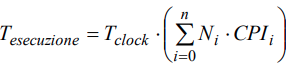
\includegraphics[width=.4\linewidth]{tempo_di_esecuzione}
	\label{fig:tempodiesecuzione} }}%
	\qquad
	\subfloat[\centering Milion Instruction Per Second]{{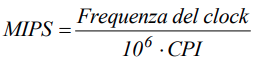
\includegraphics[width=.4\linewidth]{Milion_Instruction_Per_Second} }}%
	%\caption{2 Figures side by side}%
	\label{fig:mips}%
\end{figure}

\begin{figure}[h]%
	\centering
	\subfloat[\centering Prestazione]{{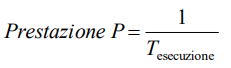
\includegraphics[width=5cm]{prestazione} }}%
	\label{fig:prestazione}
	\qquad
	\subfloat[\centering Legge di Amdhal]{{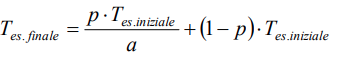
\includegraphics[width=.5\linewidth]{legge_di_amdhal} }}% prima era width=5cm
	%\caption{2 Figures side by side}%
	\label{fig:leggediamdhal}%
\end{figure}


% --- ESERCIZIO 1 MIGLIORAMENTO PRESTAZIONI MEMORIA ---

\newpage 

\begin{figure}[ht]
	%\centering
	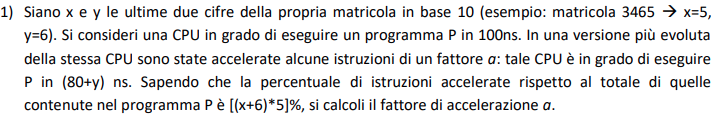
\includegraphics[width=1\linewidth]{es1_MiglioramentoPrestazioneMemoria}
	%\caption{}
	\label{fig:es1MiglioramentoPrestazioneMemoria}
\end{figure}

\textsf{{\small Esempio: matricola 3465 \textrightarrow $x = 5, y = 6$}} \break

\textsf{{\small Matricola (non la mia) = 2602}} \\
$ x = 2 $ \\
$ y = 0 $ \\

$ \text{T}_i \text{ (Tempo iniziale) } = 100 \text{ ns (nanosecondi)} $ \\

$ \text{T}_f \text{ (Tempo finale) } = 80 + y = 80 + 0 = 80 \text{ ns}$ \\

$ P = [(x + 6)\cdot 5]\% \rightarrow [(2 + 6)\cdot 5]\% = 40\% $ \\

$ \alpha = ? $ \\

\textsf{{\large Legge di Amdhal a pag.\pageref{fig:leggediamdhal}}} \\

$ \text{T}_f = \frac{\text{P}\cdot \text{T}_i}{\alpha} + (1 - p) \cdot \text{T}_i $ \\

$ 80 = \frac{0.04 \cdot 100}{\alpha} + 0,6 \cdot 100 $ \\

$ \rightarrow 80 = \frac{40}{\alpha} + 60 \rightarrow 80 - 60 = \frac{40}{\alpha} \rightarrow 20 \cdot \alpha = 40 \rightarrow \color{red}\boxed{\normalcolor\alpha = 2} $ \\

\textrm{\color{red}IL DOPPIO PIU' VELOCE} \\

% --- ESERCIZIO 2 MIGLIORAMENTO PRESTAZIONE MEMORIA ---

\begin{figure}[ht]
	%\centering
	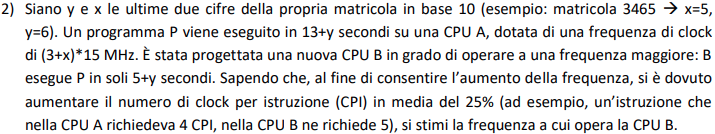
\includegraphics[width=1\linewidth]{es2_MiglioramentoPrestazioneMemoria}
	%\caption{}
	\label{fig:es2MiglioramentoPrestazioneMemoria}
\end{figure}
\enlargethispage{60pt}
\textsf{{\small Matricola = 2602}} $ (x = 2,y = 0) $\\

$ \text{T}_\text{A} = 13 \text{ s (secondi)} $ \\

$ \text{F}_\text{A} = 75 \text{ MHz (MegaHertz)} $ \\

$ \text{T}_\text{B} = 5 \text{ s} $ \\

$ \text{CPI}_\text{B} \text{ (Clock per Instruction)} = 1,25 \cdot \text{CPI}_\text{A} $ \\

$ \text{F}_\text{B} = ? $ \\

\textsf{{\large Prestazioni dei Calcolatori a pag.\pageref{fig:prestazione}}} \\

$ \text{T}_\text{ES} = \text{T}_\text{clock} \cdot \underbrace{\sum_{i = 0}^{n} \text{N}_i \cdot \text{CPI}_i} _{\text{CPI}_\text{TOT}} $ \\

\begin{itemize}
\item\textsf{{\small \textcolor{red}{$\text{T}_\text{clock}$ periodo di clock della macchina} }} \\
\item\textsf{{\small \textcolor{red}{$\text{CPI}_\text{i}$ numero di clock per istruzione di tipo i} numero di clock occorrenti affinchè avvenga l'esecuzione dell'istruzione.}} \\
\item\textsf{{\small \textcolor{red}{$\text{N}_\text{i}$ numero di istruzioni di tipo i} (somme, sottrazioni, salti, ecc..).}} \\
\end{itemize}

\pagebreak

$ \text{T}_\text{ES} \simeq \text{T}_\text{clock} \cdot \text{N}_\text{TOT} \cdot \widetilde{\text{CPI}}  $ \\

\textsf{{\small Quella tilde sopra il CPI significa "Mediamente per ogni istruzione"}} \\

$ \text{T}_\text{clock} = \frac{1}{\text{F}} $ \\

\begin{equation*}
\begin{cases}
13 = \frac{1}{75 \cdot 10^6} \cdot \text{N}_\text{TOT} \cdot\widetilde{\text{CPI}} \\
5 = \frac{1}{\text{F}_\text{B}} \cdot \text{N}_\text{TOT} \cdot \widetilde{\text{CPI}}_\text{B} \\
\end{cases}
\end{equation*}

\textsf{{\small $\text{N}_\text{TOT} $ c'è due volte perchè è lo stesso programma e quindi stesse istruzioni}}  \\

\noindent\begin{minipage}{.5\linewidth}
\begin{equation*}
\begin{cases}
13 \cdot 75 \cdot 10^6 = \text{N}_\text{TOT} \cdot \widetilde{\text{CPI}}_\text{A} \\
5 \cdot \text{F}_\text{B} = \text{N}_\text{TOT} \cdot 1,25 \cdot \widetilde{\text{CPI}}_\text{A} \\
\end{cases}
\end{equation*}
\end{minipage}
\begin{minipage}{.35\linewidth}
	\begin{equation*}
		\begin{cases}
			975 \cdot 10^6 = \text{N}_\text{TOT} \cdot \widetilde{\text{CPI}}_\text{A} \\
		    \text{F}_\text{B} = \frac{1,25 \cdot \text{\color{red}\sout{\normalcolor975}} \cdot 10^6}{\text{\color{red}\sout{\normalcolor5}}} \\
		\end{cases}
	\end{equation*}
\end{minipage}

$ \text{F}_\text{B} = 243,75 \cdot 10^6 \text{ Hz} = 243,75 \text{ Mhz} $ \\

% --- ESERCIZIO 3 MIGLIORAMENTO PRESTAZIONI MEMORIA ---

\begin{figure}[ht]
	%\centering
	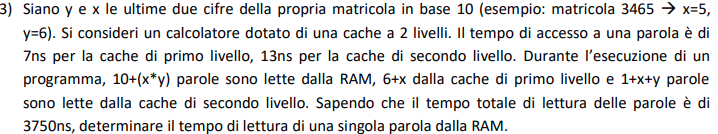
\includegraphics[width=1\linewidth]{es3_MiglioramentoPrestazioneMemoria}
	%\caption{}
	\label{fig:es3MiglioramentoPrestazioneMemoria}
\end{figure}

$ \text{MATR } = 2602 \hspace{0.1cm}(x = 2, y = 0) $ \\

$\text{T}_\text{C1} = 7 \text{ ns} $\\
$\text{T}_\text{C2} = 13 \text{ ns} $\\

\[
\begin{rcases*}
	\text{N}_\text{RAM} = 10 + (x \cdot y) \\
	\text{N}_\text{C1} = 8 \\
	\text{N}_\text{C2} = 3 \\
\end{rcases*} \text{21 ($ \text{N}_\text{TOT}$) PAROLE}
\]

$ \text{T}_\text{TOT} = 3750 \text{ ns} $ \\
$ \text{T}_\text{RAM} = ? $ \\

$ \text{T}_\text{TOT} = (\text{N}_\text{TOT} \cdot \text{T}_\text{C1}) + [(\text{N}_\text{TOT} - \text{N}_\text{C1}) \cdot \text{T}_\text{C2}] + \cdots + [(\text{N}_\text{TOT} - \text{N}_\text{C1} - \text{N}_\text{C2}) \cdot \text{T}_\text{RAM}] $ \\

\textsf{{\small Parole da cercare $(\text{N}_\text{TOT})$ , nella cache L1 $(\text{T}_\text{C1})$ , Parole da cercare meno quelle che ho già trovato nella cache 1 $(\text{N}_\text{TOT} - \text{N}_\text{C1})$}} \\

$ 3750 = 21 \cdot 7 + (21 - 8) \cdot 13 + (21 - 8 - 3) \cdot \text{T}_\text{RAM} $ \\

$ 3750 = 147 + 169 + 10 \cdot \text{T}_\text{RAM} $ \\

$ \frac{3750 - 147 - 169}{10} = \text{T}_\text{RAM} \Rightarrow \text{T}_\text{RAM} \simeq \color{red}\boxed{\normalcolor343,3 \text{ ns}} $ \\

\textsf{{\footnotesize Esercizi non necessariamente realistici.}} \\

% --- ESERCIZIO 4 MIGLIORAMENTO PRESTAZIONI MEMORIA ---

\pagebreak

\begin{figure}[ht]
	%\centering
	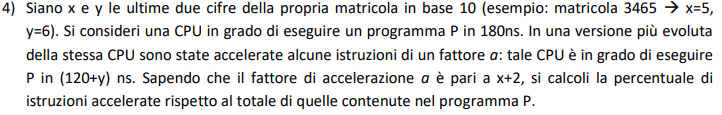
\includegraphics[width=1\linewidth]{es4_MiglioramentoPrestazioneMemoria}
	%\caption{}
	\label{fig:es4MiglioramentoPrestazioneMemoria}
\end{figure}

$ \text{MATR} = 2602 \hspace{0.1cm}(x = 2, y = 0) $ \\

$ \text{T}_\text{i} = 180 \text{ ns} $ \\
$ \text{T}_\text{F} = 120 \text{ ns} $ \\
$ \alpha = 4 $ \\

$ 120 = \frac{\text{P} \cdot \color{red}\cancel{\normalcolor180}}{\color{red}\cancel{\normalcolor4}} + (1 - \text{P}) \cdot 180 \Rightarrow 120 = \text{P} \cdot 45 + (1 - \text{P}) \cdot 180$ \\

$ 120 = \text{P} \cdot 45 + 180 - \text{P} \cdot 180 $ \\

$ 120 = \text{P}(45 - 180) + 180 $ \\

$ \frac{120 - 180}{45 - 180} = \text{P}  \Rightarrow \text{P} = \frac{-60}{-135} \simeq \color{red}\boxed{\normalcolor 44,4\%} $ \\

\textsf{{\small Andava bene anche tenere la frazione semplificata ($ \frac{\text{\color{red}\sout{\normalcolor-60}}}{\text{\color{red}\sout{\normalcolor-135}}} = \frac{\color{red}\cancel{\normalcolor12}}{\color{red}\cancel{\normalcolor22}} = \frac{4}{9}$) al posto di scriverlo in percentuale.}} \\

% --- ESERCIZIO 5 MIGLIORAMENTO PRESTAZIONI MEMORIA ---

\begin{figure}[ht]
	%\centering
	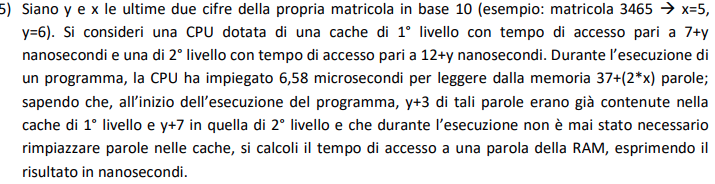
\includegraphics[width=1\linewidth]{es5_MiglioramentoPrestazioneMemoria}
	%\caption{}
	\label{fig:es5MiglioramentoPrestazioneMemoria}
\end{figure}

\textsf{{\small Non è mai stato necessario rimpiazzare parole nella cache = cache non variano.}} \\

$ \text{MATR} = 2602 \hspace{.1cm}(x = 2, y = 0) $ \\

$ \text{T}_\text{C1} = 7 \text{ ns} $ \\
$ \text{T}_\text{C2} = 12 \text{ ns} $ \\
$ \text{T}_\text{TOT} = 6,58 \overset{10^-6}{\text{ ms (millisecondi)}} = 6580 \overset{10^-9}{\text{ ns (nanosecondi)}} $ \\

$ \text{N}_\text{TOT} = 41 $ \\
$ \text{N}_\text{C1} = 3 $ \\
$ \text{N}_\text{C2} = 7 $ \\
$ \text{T}_\text{RAM} = ? $ \\

$ 6580 = 41 \cdot 7 + (41 - 3) \cdot 12 + (41 - 3 - 7) \cdot \text{T}_\text{RAM} $ \\
$ 6580 = 287 + 38 \cdot 12 + 31 \cdot \text{T}_\text{RAM} $ \\
$ 6580 = 287 + 456 + 31 \cdot \text{T}_\text{RAM} $ \\

$ \frac{6580 - 287 - 456}{31} = \text{T}_\text{RAM} $ \\

$ \text{T}_\text{RAM} = \frac{5837}{31} \simeq \color{red}\boxed{\normalcolor188,3 \text{ ns}} $ \\

% --- ESERCIZIO 6 MIGLIORAMENTO PRESTAZIONI MEMORIA ---

\newpage

\begin{figure}[ht]
	%\centering
	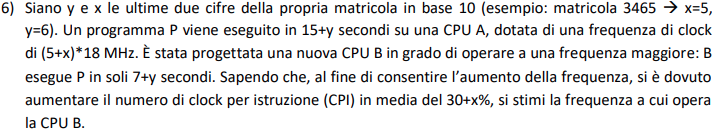
\includegraphics[width=1\linewidth]{es6_MiglioramentoPrestazioneMemoria}
	%\caption{}
	\label{fig:es6MiglioramentoPrestazioneMemoria}
\end{figure}

$ \text{MATR} = 2602 \hspace{.1cm}(x = 2, y = 0) $ \\

$ \text{T}_\text{A} = 15 \text{ s} $ \\
$ \text{F}_\text{A} = 126 \text{ Mhz} $ \\
$ \text{T}_\text{B} = 7 + y \text{ secondi} $ \\
$ \text{CPI}_\text{B} = 1,32 \cdot \text{CPI}_\text{A} $ \\
$ \text{F}_\text{B} = ? $ \\

\noindent\begin{minipage}{.5\linewidth}
\begin{equation*}
\begin{cases}
15 = \frac{1}{126 \cdot 10^6} \cdot \text{N}_\text{TOT} \cdot \widetilde{\text{CPI}_\text{A}} \\
7 = \frac{1}{\text{F}_\text{B}} \cdot \text{N}_\text{TOT} \cdot \widetilde{\text{CPI}_\text{B}} \\
\end{cases}
\end{equation*}
\end{minipage}
\begin{minipage}{.35\linewidth}
\begin{equation*}
	\begin{cases}
		15 \cdot 126 \cdot 10^6 = \text{N}_\text{TOT} \cdot \widetilde{\text{CPI}_\text{A}} \\
		7 \cdot \text{F}_\text{B} = \text{N}_\text{TOT} \cdot 1,32 \cdot \widetilde{\text{CPI}_\text{A}} \\
	\end{cases}
\end{equation*}
\end{minipage}

\begin{equation*}
\begin{cases}
1890 \cdot 10^6 = \text{N}_\text{TOT} \cdot \widetilde{\text{CPI}_\text{A}} \\
\text{F}_\text{B} = \frac{1890 \cdot 10^6 \cdot 1,32}{7} \\
\end{cases}
\end{equation*}

$ \text{F}_\text{B} \simeq 356,4 \cdot 10^6 \text{ hz} = \color{red}\boxed{\normalcolor 356,4 \text{ Mhz}} $ \\

% --- CONCLUSIONI ---

\newpage

\section{Conclusioni}

\flushright
\date{13, Dicembre 2020} \break

\centering

\textsf{{\normalsize In questo documento/articolo ho raccolto tutti o quasi gli esercizi svolti durante il corso di "Architetture degli Elaboratori" tranne alcuni che non ho scritto (come la Prova di Autovalutazione).}} \\

\textsf{{\normalsize Al momento ho concluso questo documento/articolo. \\ Ma in futuro, potreì aggiungere degli esercizi, in fondo, su tutti gli argomenti \\
		e poi le soluzioni a questi.}} \\
	
\textsf{{\normalsize Inoltre potreì anche mostrare i miei esercizi in Assembly che ho consegnato.}} \break


\flushleft
\large
%$ \mathfrak{Luca} $

\begin{comment}
\closing{Yours faithfully,\\
	\fromsig{\includegraphics[scale=1]{signature.jpg}} \\
	\fromname{Your name}
}
\end{comment}

%Le prime quattro non vanno, perchè il package emerald is not found
%JD: {\ECFJD\setul{0.1ex}{}\ul{~~John Quegpylf Doe~~}}

%Skeetch: {\ECFSkeetch\setul{0.1ex}{}\ul{~~John Quegpylf Doe~~}}

%Teen Spirit: {\ECFTeenSpirit\setul{-0.1ex}{0.3pt}\ul{~~John Quegpylf Doe~~}}

%Tall Paul: {\ECFTallPaul\setul{0.15ex}{}\ul{~~John Quegpylf Doe~~}}

Firma: {\cursive\setul{0.1ex}{}\ul{~~Luca~~}}

%Firma: {\iminfamily\setul{0.1ex}{}\ul{~~Luca~~}}